% !TEX root = ../Dokumentation.tex
\subsection{Fahrbahnerkennung}
\textbf{Funktionsbeschrieb}
Die Fahrbahnerkennung soll primär mittels Kamera umgesetzt werden. Dazu werden Bilder aus dem zu Verfügung gestellten Bilderpool entnommen, in Graustufen umgewandelt und anschliessend einer Kantenanalyse unterzogen. Dazu wird ein eigener Algorithmus verwendet, der jeweils eine Bildzeile als Graph einer Funktion $y = f(x)$ angeschaut, wobei $x$ der Pixelkoordinate der Spalte und $y$ dem Graustufenwert des Pixels entspricht.\\
Anhand der vorhandenen Informationen kann die Fahrbahn und demzufolge während der Fahrt der Korrekturvektor ermittelt werden. Die Korrektur selber soll mittels PID-Regelung realisiert werden, um eine ruhige Fahrt zu erreichen.
\textbf{Komponentenbeschrieb}
\begin{figure}[h!]%Position festigen
\centering
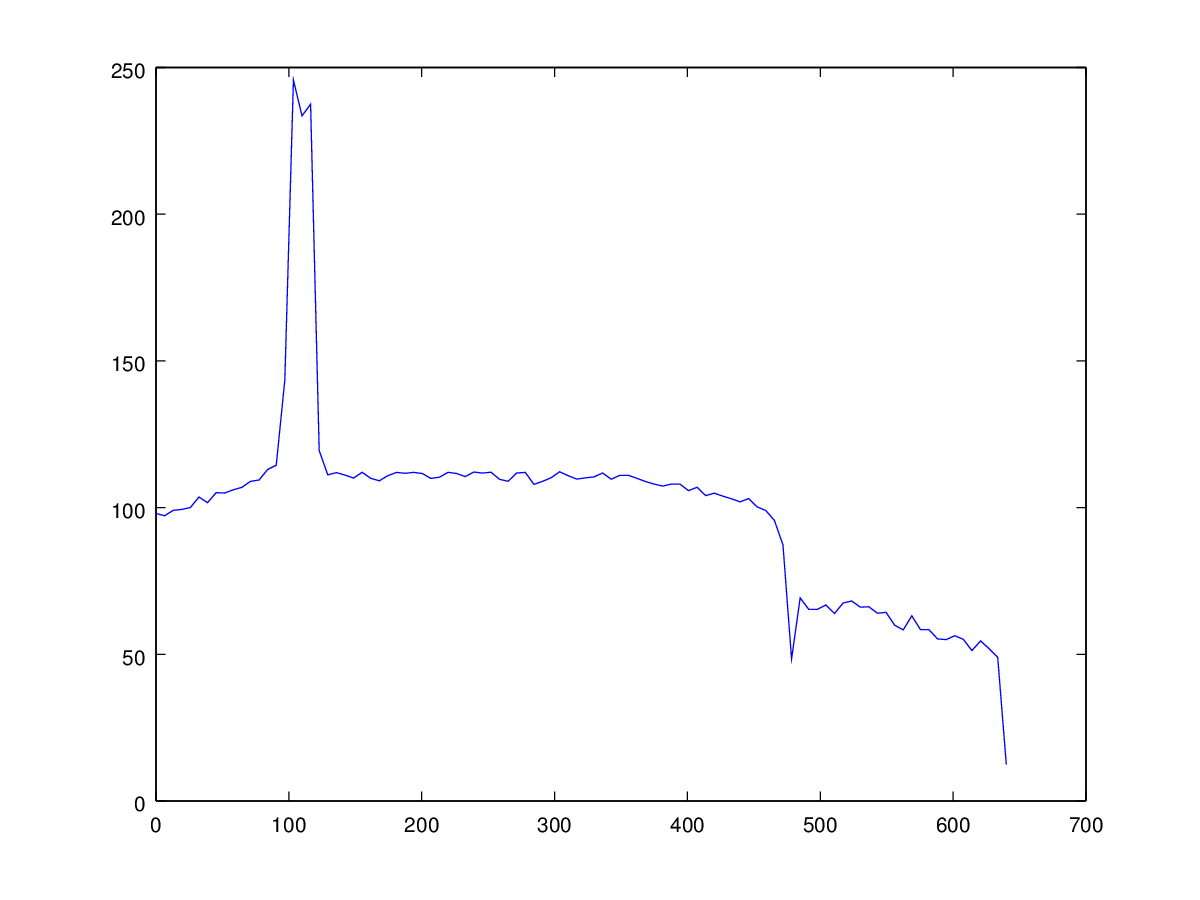
\includegraphics[width=0.3\textwidth]{pictures/graphPicture.png}
\caption{Graph der Graustufenwerte einer Bilderzeile}
\label{fig:OpenCV}
\end{figure}
\textbf{Begründung}
Wenn benötigt
\textbf{Berechnungen}
\textbf{Testergebnisse}